% Beamer Presentation and Lecture Note Template
% Version 0.1
% by Paul Vesey

%%%%%%%%%%%%%%%%%%%%%%%%%%%%%%%%%%%%%
% Switch between these for presentation
% and A4 Lecture Notes
%\documentclass[ignorenonframetext,red]{beamer}     % use this for presentations and slide handouts
%\documentclass[ignorenonframetext]{beamer}     % use this for presentations and slide handouts
%\documentclass[a4paper]{article}     % use this to print the notes

%\documentclass{beamer}

%%%%%%%%%%%%%%%%%%%%%%%%%%%%%%%%%%%%%%%%
% Turn off all of these for A4 Notes
%
\mode<presentation> {
%\usetheme{lankton-keynote} % Seperate Download
%\usetheme{Madrid}
\usetheme{Antibes}
\setbeamercovered{invisible}
\setbeamertemplate{navigation symbols}{} 
}

%%\mode<presentation>{}



%%%%%%%%%%%%%%%%%%%%%%%%%%%%%%%%%%%%%%%%%%
%%%%%%%%%%%%%%%%%%%%%%%%%%%%%%%%%%%%%%%%%%

\usepackage{eurosym}
\usepackage{graphicx}
\usepackage{wasysym}
\usepackage{listings}
\usepackage{pxfonts}
\usepackage{verbatim}
\usepackage{color}
\usepackage{xcolor}
\usepackage{wrapfig}
\usepackage{hyperref}
\usepackage[nomain, xindy, toc, acronym]{glossaries}
\include{refs/glossary}
\include{refs/acronyms}

\makeglossaries{}
\usepackage[xindy]{imakeidx}
\makeindex




%%%%%%%%%%%%%%%%%%%%%%%%%%%%%%%%%%%%%%%%%%%%%%%%%%%%%%
%%%%%%%%%%%%%%%%%%%%%%%%%%%%%%%%%%%%%%%%%%%%%%%%%%%%%%
%
%THIS IS FOR PRINTING SLIDE HANDOUTS
%\usepackage{pgfpages}
%\pgfpagesuselayout{2 on 1}[a4paper,border shrink=5mm]

%%%%%%%%%%%%%%%%%%%%%%%%%%%%%%%%%%%%%%%%%%%%%%%%%%%%%%%
%%%%%%%%%%%%%%%%%%%%%%%%%%%%%%%%%%%%%%%%%%%%%%%%%%%%%%
%
%THIS IS FOR PRINTING A4 NOTES
%
%\usepackage{beamerarticle}    % Turn this on for A4 notes

%%%%%%%%%%%%%%%%%%%%%%%%%%%%%%%%%%%%%%%%%%%%%%%%%%%%%%

%\renewcommand\verbatim@font{\color{red}\normalfont\ttfamily}




%\usepackage{bm} 
% For typesetting bold math (not \mathbold)
%\logo{\includegraphics[height=0.6cm]{yourlogo.eps}}
%
\title[Advanced Graphics \& Visualisation]{Advanced Graphics \& Visualisation}
%
\author{Paul Vesey}
\institute[LIT]
{
Limerick Institute of Technology \\
\medskip
{\emph{paul.vesey@lit.ie}}
}
\date{2014-2015}
% \today will show current date. 
% Alternatively, you can specify a date.

\begin{document}
%

%\lstset{language=C++, frame=single}

\lstset{language=HTML,
				basicstyle=\small,
				breaklines=true,
        numbers=left,
        numberstyle=\tiny,
        showstringspaces=false,
        aboveskip=-20pt,
        frame=leftline
        }



\tableofcontents
\newpage



\begin{frame}
\titlepage
\end{frame}\begin{center}\line(1,0){250}\end{center}
%
%


\section{Introduction}




\begin{frame}
\frametitle{About me}
\begin{itemize}
	\item Paul Vesey
	\item 13B09
	\item email is best
\end{itemize}

\end{frame}
\begin{center}\line(1,0){250}\end{center}







\begin{frame}
\frametitle{The course in a nutshell}
\begin{itemize}
	\item Technology
	\item Composition \& Image Creation
	\item Digital Images
	\item Digital Video \& Game Engine
\end{itemize}
\end{frame}\begin{center}\line(1,0){250}\end{center}


 
 \begin{frame}
\frametitle{Learning Outcomes}
On successful completion of this module the learner will/should be able to\ldots
\begin{enumerate}
	\item Understand the hardware and software technology requirements for advanced visualization.
	\item Understand image composition, DOF, color, hue, and other image characteristics.
	\item Develop and critique photo-realistic rendered images of building interior and exteriors.
	\item Develop professional level video animations of virtual environments.
\end{enumerate}
\end{frame}
\begin{center}\line(1,0){250}\end{center}



\begin{frame}
\frametitle{Indicative Syllabus \hfill\hfill Technology}

\begin{itemize}
	\item Hardware and Software
	\item Ray Tracing, Graphics Processors, Memory, Distributed Processing
	\item Rendering Engines and Methods
	\item Compression Technologies and File Types
\end{itemize}
\end{frame}
\begin{center}\line(1,0){250}\end{center}



\begin{frame}
\frametitle{Indicative Syllabus \hfill\hfill Composition \& Image Creation}

\begin{itemize}
	\item Pattern, Symmetry, Texture, Depth of Field, Lines
	\item Lens Characteristics, Lighting Characteristics, 
	\item Dominance \& Subordination, Unity, Coherence, Positive \& Negative Space
	\item Balance, Shutter, Aperture, Light Measurement, Focus
\end{itemize}
\end{frame}
\begin{center}\line(1,0){250}\end{center}


\begin{frame}
\frametitle{Indicative Syllabus \hfill\hfill Digital Images}

\begin{itemize}
	\item Material Creation, Editing and Applicaiton
	\item Texture Creation, Editing and Application
	\item Cameras, Simulated Lighting, Artistic Lighting
	\item Post Processing, RPC Content
\end{itemize}
\end{frame}
\begin{center}\line(1,0){250}\end{center}


\begin{frame}
\frametitle{Indicative Syllabus \hfill\hfill Digital Video \& Game Engine}

\begin{itemize}
	\item Animation and Production Process
	\item Video Editing, Effects, and Audio
	\item Game Environments, Asset Creation and Management
	\item Controller Technologies
\end{itemize}
\end{frame}
\begin{center}\line(1,0){250}\end{center}






\begin{frame}
\frametitle{Assessment}
\textbf{100\% Continuous Assessment}
\begin{table}[htp]
	\centering
		\begin{tabular}{|l|l|}
			\hline
			\textbf{Assessment} & \textbf{Proportion} \\
			\hline
			Collection of photo-realistic images &		35\% \\
			5 minute animated video 						&   	35\% 			\\
			End of Year Integrated Project (Studio)  & 30\% 		\\
			\hline
		\end{tabular}
		\label{tab:Assessments}
\end{table}
\begin{itemize}
	\item The End of Year Project will be integrated into the studio project deliverables\\
	\item There will be numerous application studies throughout the year that will count towards each assessment.
\end{itemize}
\end{frame}
\begin{center}\line(1,0){250}\end{center}





\begin{table}[htp]
	\centering
		\scalebox{1.0}{
		\begin{tabular}{|c|r|l|}
			\hline
			\textbf{Week} & \textbf{Date } & \textbf{Activity}	\\
			\hline
			1		&	15/9	& Intro / Revit Revision				\\	
			2		&	22/9	& Revit Revision 								\\	
			3		&	29/9	& Revit	to Unity 3D							\\	
			4		&	6/10	& Unity 3D Workflow							\\	
			5		&	13/10	& Unity 3D Terrain 							\\	
			6		&	20/10	& Unity 3D Controllers					\\	
			7		&	26/10	& Bank Holiday									\\	
			8		&	3/11	& 								\\	
			9 	&	10/11	& 								\\	
			10	&	17/11	& 								\\
			11	&	24/11	& 								\\
			12	&	1/12	& 	\\
			
			
			13	&	8/12	& Christmas Exams								\\
					& 			& \textbf{Christmas Break}			\\
			14	& 5/1		&		\\
			15	& 12/1	&				\\
			16	& 19/1	&					\\
			17	& 26/1	&							\\										
			18	& 2/2		&							\\
			19	& 9/2		&	(Float)												\\
			20	& 16/2	&	 	\\
			21	& 23/2	&												\\										
			22	& 2/3		&										\\
			23	& 9/3		&											\\									
			24	& 16/3	&											\\
			25	& 23/3	&											\\										
				  & 			& \textbf{Easter Break}					\\
			26	& 13/4	&	EoY Project Support						\\
			27	& 20/4	&	EoY Project Support						\\									
			28	& 27/4	&	Presentations									\\
				  & 4/5		& Revision/Exam Week 						\\			
			\hline
		\end{tabular}}
				\label{tab:LessonPlanLong}
\end{table}




\section{Image Composition and Critique}



\begin{frame}
\frametitle{Composition}
\begin{itemize}
	\item Images should tell a story, engage the viewer, or elicit an emotional response.
	\item Images of interior design should do the same.
	\item ID images tend to fall into the documentary variety; there is no reason why ID images cannot be as engaging and exciting as other schools.
\end{itemize}
\end{frame}
\begin{center}\line(1,0){250}\end{center}


\begin{frame}
\frametitle{Emotion}
\begin{figure}
	\centering
		\includegraphics[width=8cm]{img/2091078908.jpg}
	\caption{TEST Image}
	\label{fig:lightingtypes}
\end{figure}
\end{frame}
\begin{center}\line(1,0){250}\end{center}


\begin{frame}
\frametitle{Emotion}
\begin{figure}
	\centering
		\includegraphics[width=10cm]{img/DERREN-BROWN.jpg}
	\caption{Derren Brown}
	\label{fig:lightingtypes}
\end{figure}
\end{frame}
\begin{center}\line(1,0){250}\end{center}



\begin{frame}
\frametitle{Emotion}
\begin{figure}
	\centering
		\includegraphics[width=9cm]{img/whitesNonWhites.jpg}
	\caption{Elliott Erwitt - North Carolina in 1950}
	\label{fig:lightingtypes}
\end{figure}
\end{frame}
\begin{center}\line(1,0){250}\end{center}





\begin{frame}
\frametitle{Tell a Story or Capture a Moment}
\begin{figure}
	\centering
		\includegraphics[width=7cm]{img/18-Raphael-Paintings.jpg}
	\caption{Raphael - The Entombment (1508)}
	\label{fig:lightingtypes}
\end{figure}
\end{frame}
\begin{center}\line(1,0){250}\end{center}




\begin{frame}
\frametitle{Tell a Story or Capture a Moment}
\begin{figure}
	\centering
		\includegraphics[width=5cm]{img/DurerAngelBoy.jpg}
	\caption{TEST Image}
	\label{fig:lightingtypes}
\end{figure}
\end{frame}
\begin{center}\line(1,0){250}\end{center}




\begin{frame}
\frametitle{Tell a Story or Capture a Moment}
\begin{figure}
	\centering
		\includegraphics[width=5cm]{img/Durerfurleger.jpg}
	\caption{Albrecht Dürer - Weeping Angel Boy (1521)}
	\label{fig:lightingtypes}
\end{figure}
\end{frame}
\begin{center}\line(1,0){250}\end{center}




\begin{frame}
\frametitle{Tell a Story or Capture a Moment}
\begin{figure}
	\centering
		\includegraphics[width=5cm]{img/DurerLotandDaughters.jpg}
	\caption{Albrecht Dürer - Lot and his Daughters (c.1496/1499}
	\label{fig:lightingtypes}
\end{figure}
\end{frame}
\begin{center}\line(1,0){250}\end{center}




\begin{frame}
\frametitle{Tell a Story or Capture a Moment}
\begin{figure}
	\centering
		\includegraphics[width=8cm]{img/nastag12.jpg}
	\caption{Sandro Botticelli - The Story of Nastagio degli Onesti (c.1483)}
	\label{fig:lightingtypes}
\end{figure}
\end{frame}
\begin{center}\line(1,0){250}\end{center}



\begin{frame}
\frametitle{Use Light to direct attention}
\begin{figure}
	\centering
		\includegraphics[width=9cm]{img/TurnerFishingBoatsStorm.jpg}
	\caption{William Turner - Dutch Fishing Boats in a Storm (1801)}
	\label{fig:lightingtypes}
\end{figure}
\end{frame}
\begin{center}\line(1,0){250}\end{center}



\begin{frame}
\frametitle{Use Light to direct attention}
\begin{figure}
	\centering
		\includegraphics[width=10cm]{img/TurnerCoal-by-Moonlight.jpg}
	\caption{William Turner - Keelmen Heaving in Coals by Moonlight (1835)}
	\label{fig:lightingtypes}
\end{figure}
\end{frame}
\begin{center}\line(1,0){250}\end{center}




\begin{frame}
\frametitle{Use Light to direct attention}
\begin{figure}
	\centering
		\includegraphics[width=8cm]{img/starry-night-VanGogh.jpg}
	\caption{Vincent van Gogh - The Starry Night (1889)}
	\label{fig:lightingtypes}
\end{figure}
\end{frame}
\begin{center}\line(1,0){250}\end{center}







\begin{frame}
\frametitle{Suggest a Story}
\begin{figure}
	\centering
		\includegraphics[width=5cm]{img/DorethaLange.jpg}
	\caption{TEST Image}
	\label{fig:lightingtypes}
\end{figure}
\end{frame}
\begin{center}\line(1,0){250}\end{center}


\begin{frame}
\frametitle{Suggest a Story}
\begin{figure}
	\centering
		\includegraphics[width=5cm]{img/DorethaLange2.jpg}
	\caption{Dorothea Lange}
	\label{fig:lightingtypes}
\end{figure}
\end{frame}
\begin{center}\line(1,0){250}\end{center}



\begin{frame}
\frametitle{Suggest a Story}
\begin{figure}
	\centering
		\includegraphics[width=8cm]{img/DorethaLange3.jpg}
	\caption{Dorothea Lange}
	\label{fig:lightingtypes}
\end{figure}
\end{frame}
\begin{center}\line(1,0){250}\end{center}





\begin{frame}
\frametitle{Who Lives Here?}
\begin{figure}
	\centering
		\includegraphics[width=8cm]{img/A.jpg}
	\caption{TEST Image}
	\label{fig:lightingtypes}
\end{figure}
\end{frame}
\begin{center}\line(1,0){250}\end{center}



\begin{frame}
\frametitle{Who Lives Here?}
\begin{figure}
	\centering
		\includegraphics[width=8cm]{img/A1.jpg}
	\caption{TEST Image}
	\label{fig:lightingtypes}
\end{figure}
\end{frame}
\begin{center}\line(1,0){250}\end{center}



\begin{frame}
\frametitle{Who Lives Here?}
\begin{figure}
	\centering
		\includegraphics[width=8cm]{img/B.jpg}
	\caption{TEST Image}
	\label{fig:lightingtypes}
\end{figure}
\end{frame}
\begin{center}\line(1,0){250}\end{center}



\begin{frame}
\frametitle{Who Lives Here?}
\begin{figure}
	\centering
		\includegraphics[width=8cm]{img/C.jpg}
	\caption{TEST Image}
	\label{fig:lightingtypes}
\end{figure}
\end{frame}
\begin{center}\line(1,0){250}\end{center}



\begin{frame}
\frametitle{Who Lives Here?}
\begin{figure}
	\centering
		\includegraphics[width=8cm]{img/D.jpg}
	\caption{TEST Image}
	\label{fig:lightingtypes}
\end{figure}
\end{frame}
\begin{center}\line(1,0){250}\end{center}



\begin{frame}
\frametitle{Who Lives Here?}
\begin{figure}
	\centering
		\includegraphics[width=8cm]{img/E.jpg}
	\caption{TEST Image}
	\label{fig:lightingtypes}
\end{figure}
\end{frame}
\begin{center}\line(1,0){250}\end{center}




\begin{frame}
\frametitle{Who Lives Here?}
\begin{figure}
	\centering
		\includegraphics[width=8cm]{img/F.jpg}
	\caption{TEST Image}
	\label{fig:lightingtypes}
\end{figure}
\end{frame}
\begin{center}\line(1,0){250}\end{center}




\begin{frame}
\frametitle{Who Lives Here?}
\begin{figure}
	\centering
		\includegraphics[width=8cm]{img/G.jpg}
	\caption{TEST Image}
	\label{fig:lightingtypes}
\end{figure}
\end{frame}
\begin{center}\line(1,0){250}\end{center}




\begin{frame}
\frametitle{Who Lives Here?}
\begin{figure}
	\centering
		\includegraphics[width=8cm]{img/H.jpg}
	\caption{TEST Image}
	\label{fig:lightingtypes}
\end{figure}
\end{frame}
\begin{center}\line(1,0){250}\end{center}




\begin{frame}
\frametitle{Who Lives Here?}
\begin{figure}
	\centering
		\includegraphics[width=8cm]{img/H.png}
	\caption{TEST Image}
	\label{fig:lightingtypes}
\end{figure}
\end{frame}
\begin{center}\line(1,0){250}\end{center}



\begin{frame}
\frametitle{Who Lives Here?}
\begin{figure}
	\centering
		\includegraphics[width=8cm]{img/J.jpg}
	\caption{TEST Image}
	\label{fig:lightingtypes}
\end{figure}
\end{frame}
\begin{center}\line(1,0){250}\end{center}



\begin{frame}
\frametitle{Who Lives Here?}
\begin{figure}
	\centering
		\includegraphics[width=8cm]{img/K.jpg}
	\caption{TEST Image}
	\label{fig:lightingtypes}
\end{figure}
\end{frame}
\begin{center}\line(1,0){250}\end{center}



\begin{frame}
\frametitle{User Story}
\begin{itemize}
	\item A user story is a simple way of describing how we expect a user to interact with the space we have created.
	\item It is a common design technique; used in early stage design to create a better understanding of the design functionality requirements
	\item In our case we are going to use this technique to develop images that will sit well with our clients
\end{itemize}
\end{frame}
\begin{center}\line(1,0){250}\end{center}



\begin{frame}
\frametitle{User Story \hfill\hfill Typical Components}
\begin{itemize}
	\item Demographic Profile; Age, Sex, etc.
	\item Space Usage; how will the user interact with this space; what will they do, when, how often, etc.
	\item By understanding these elements, we can create images that feed into the users expectations.
	\item We can give them names, family, or anything else that will allow us to develop a better understanding of their needs.
\end{itemize}
\end{frame}
\begin{center}\line(1,0){250}\end{center}



\begin{frame}
\frametitle{User Story \hfill\hfill Typical Components}
\begin{itemize}
	\item Demographic Profile; Age, Sex, etc.
	\item Space Usage; how will the user interact with this space; what will they do, when, how often, etc.
	\item By understanding these elements, we can create images that feed into the users expectations.
	\item We can give them names, family, or anything else that will allow us to develop a better understanding of their needs.
\end{itemize}
\end{frame}
\begin{center}\line(1,0){250}\end{center}





\begin{frame}
\frametitle{User Story \hfill\hfill Example}
\begin{itemize}
	\item Robert and Georgina have been married for 3 years.  They intend to have children, but not for a few years.  They have good jobs and have a reasonable disposable income.  They like living in the city but prefer the great outdoors.  They recently inherited some land, and would like to build a weekend home.  They are adamant that their new home must blend in with the landscape, and be capable of expansion when children arrive.
\end{itemize}
\end{frame}
\begin{center}\line(1,0){250}\end{center}


\begin{frame}
\frametitle{User Story Result}
\begin{figure}
	\centering
		\includegraphics[width=10cm]{img/cabana_01_large.jpg}
	\caption{TEST Image}
	\label{fig:lightingtypes}
\end{figure}
\end{frame}
\begin{center}\line(1,0){250}\end{center}


\section{Color Temperature}

\begin{frame}
\frametitle{Color Temperature}
\begin{itemize}
	\item Color Temperature refers to the color cast generated by various types of lighting
	\item In digital photography it is often referred to as 'White Balance'.
	\item Incandecent lamps tend to project warm colors; LED and florescent lamps tend to have a cold cast.
	\item The color temperature scale is Kelvin
	\item Lower color temps are warm, higher color temps are cold
\end{itemize}
\end{frame}
\begin{center}\line(1,0){250}\end{center}

\begin{frame}
\frametitle{Color Temperature}
\begin{itemize}
	\item 5000K is fairly neutral
	\item Incandescent lamps are about 3000K
	\item Florescent lamps can be about 6000K
\end{itemize}
\end{frame}
\begin{center}\line(1,0){250}\end{center}



\begin{frame}
\frametitle{3000 Kelvin}
\begin{figure}
	\centering
		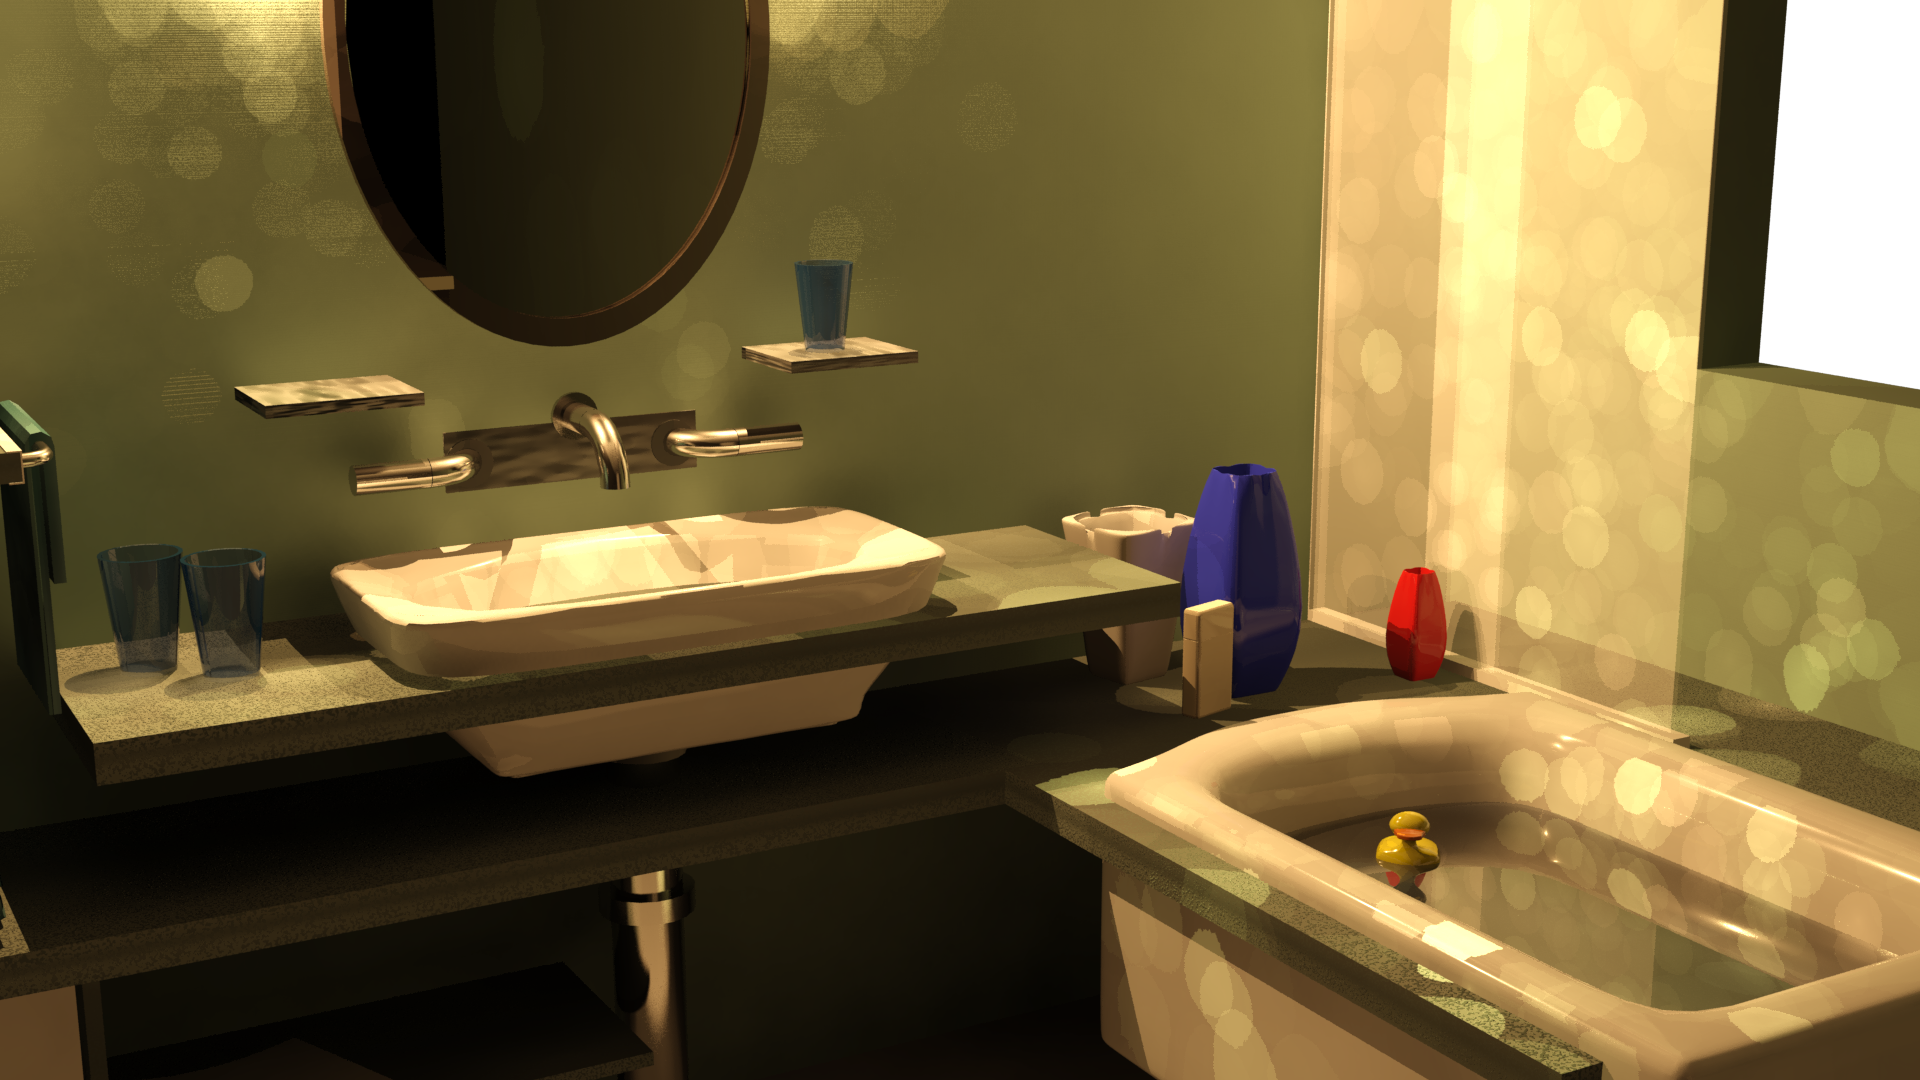
\includegraphics[width=10cm]{img/3000K.png}
	\caption{3000K}
	\label{fig:colortemp3000}
\end{figure}
\end{frame}
\begin{center}\line(1,0){250}\end{center}


\begin{frame}
\frametitle{5000 Kelvin}
\begin{figure}
	\centering
		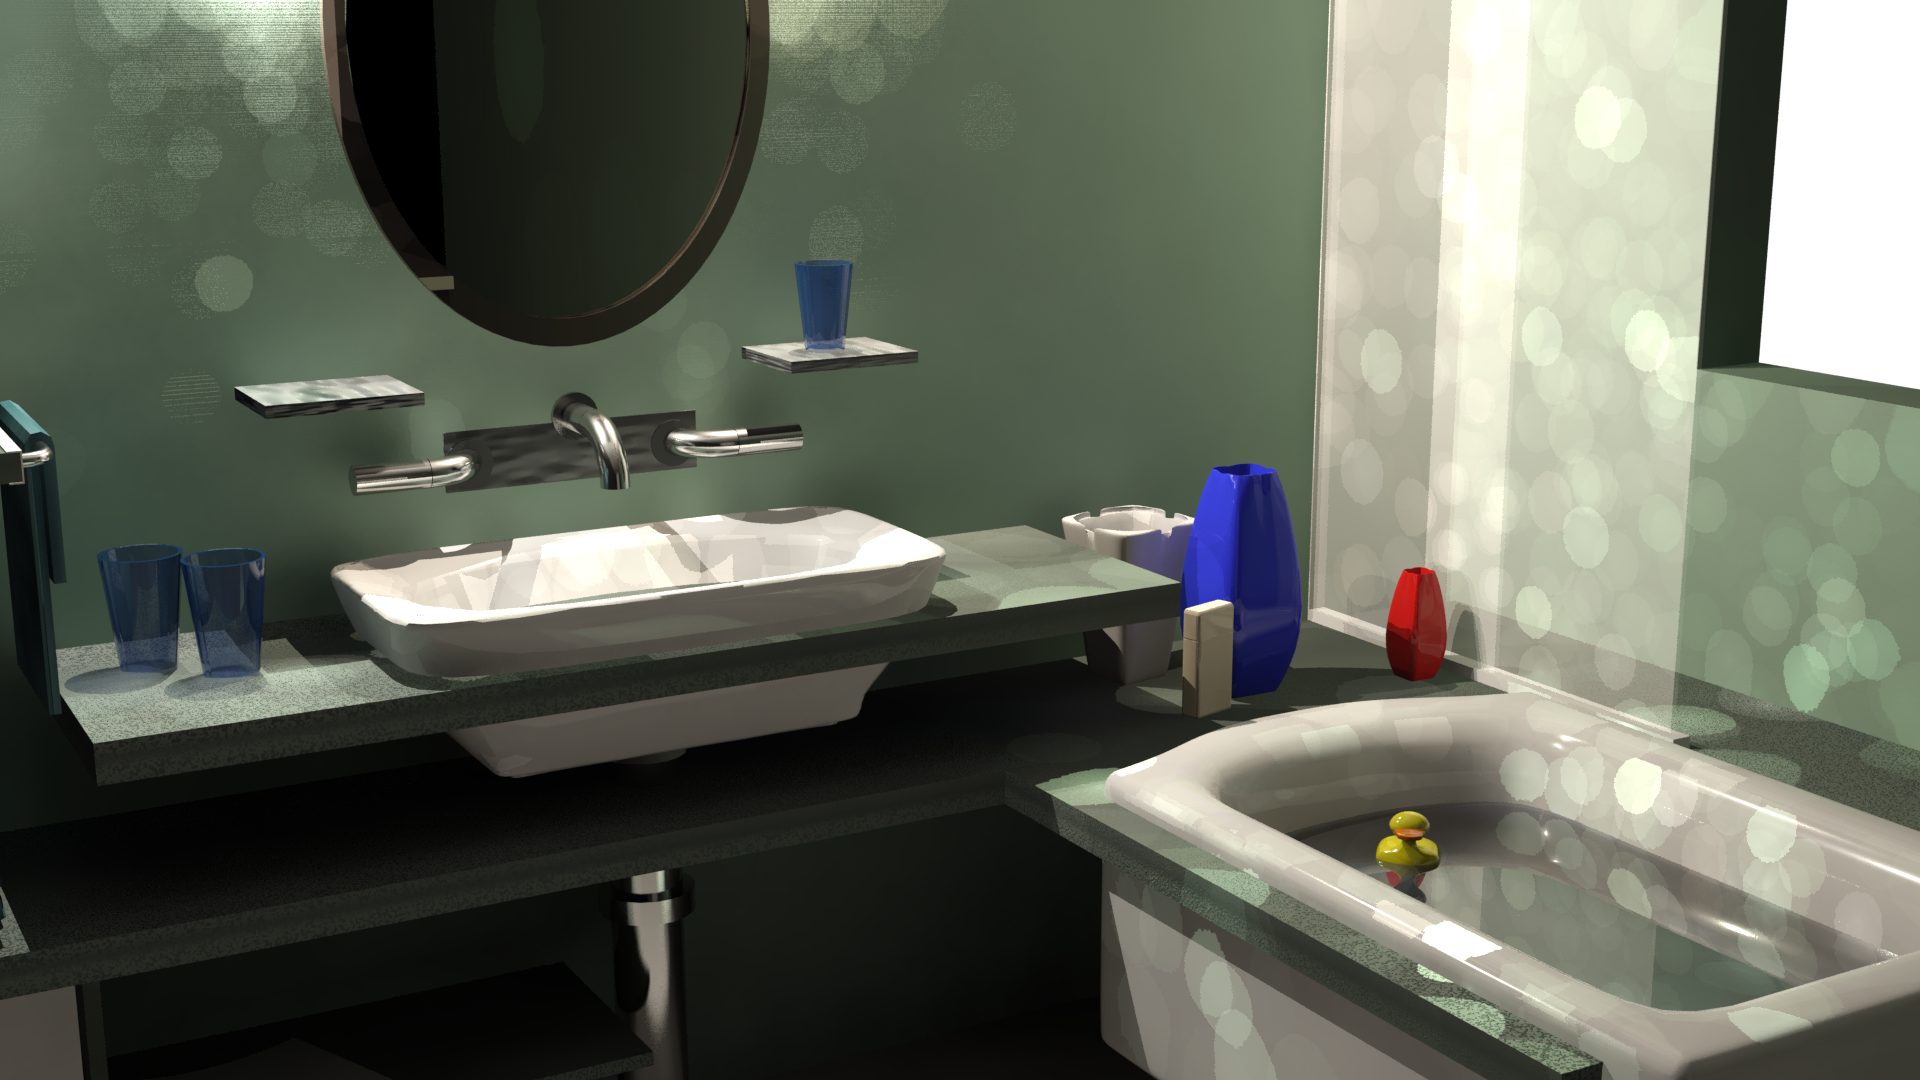
\includegraphics[width=10cm]{img/5000K.png}
	\caption{5000K}
	\label{fig:colortemp5000}
\end{figure}
\end{frame}
\begin{center}\line(1,0){250}\end{center}

\begin{frame}
\frametitle{8000 Kelvin}
\begin{figure}
	\centering
		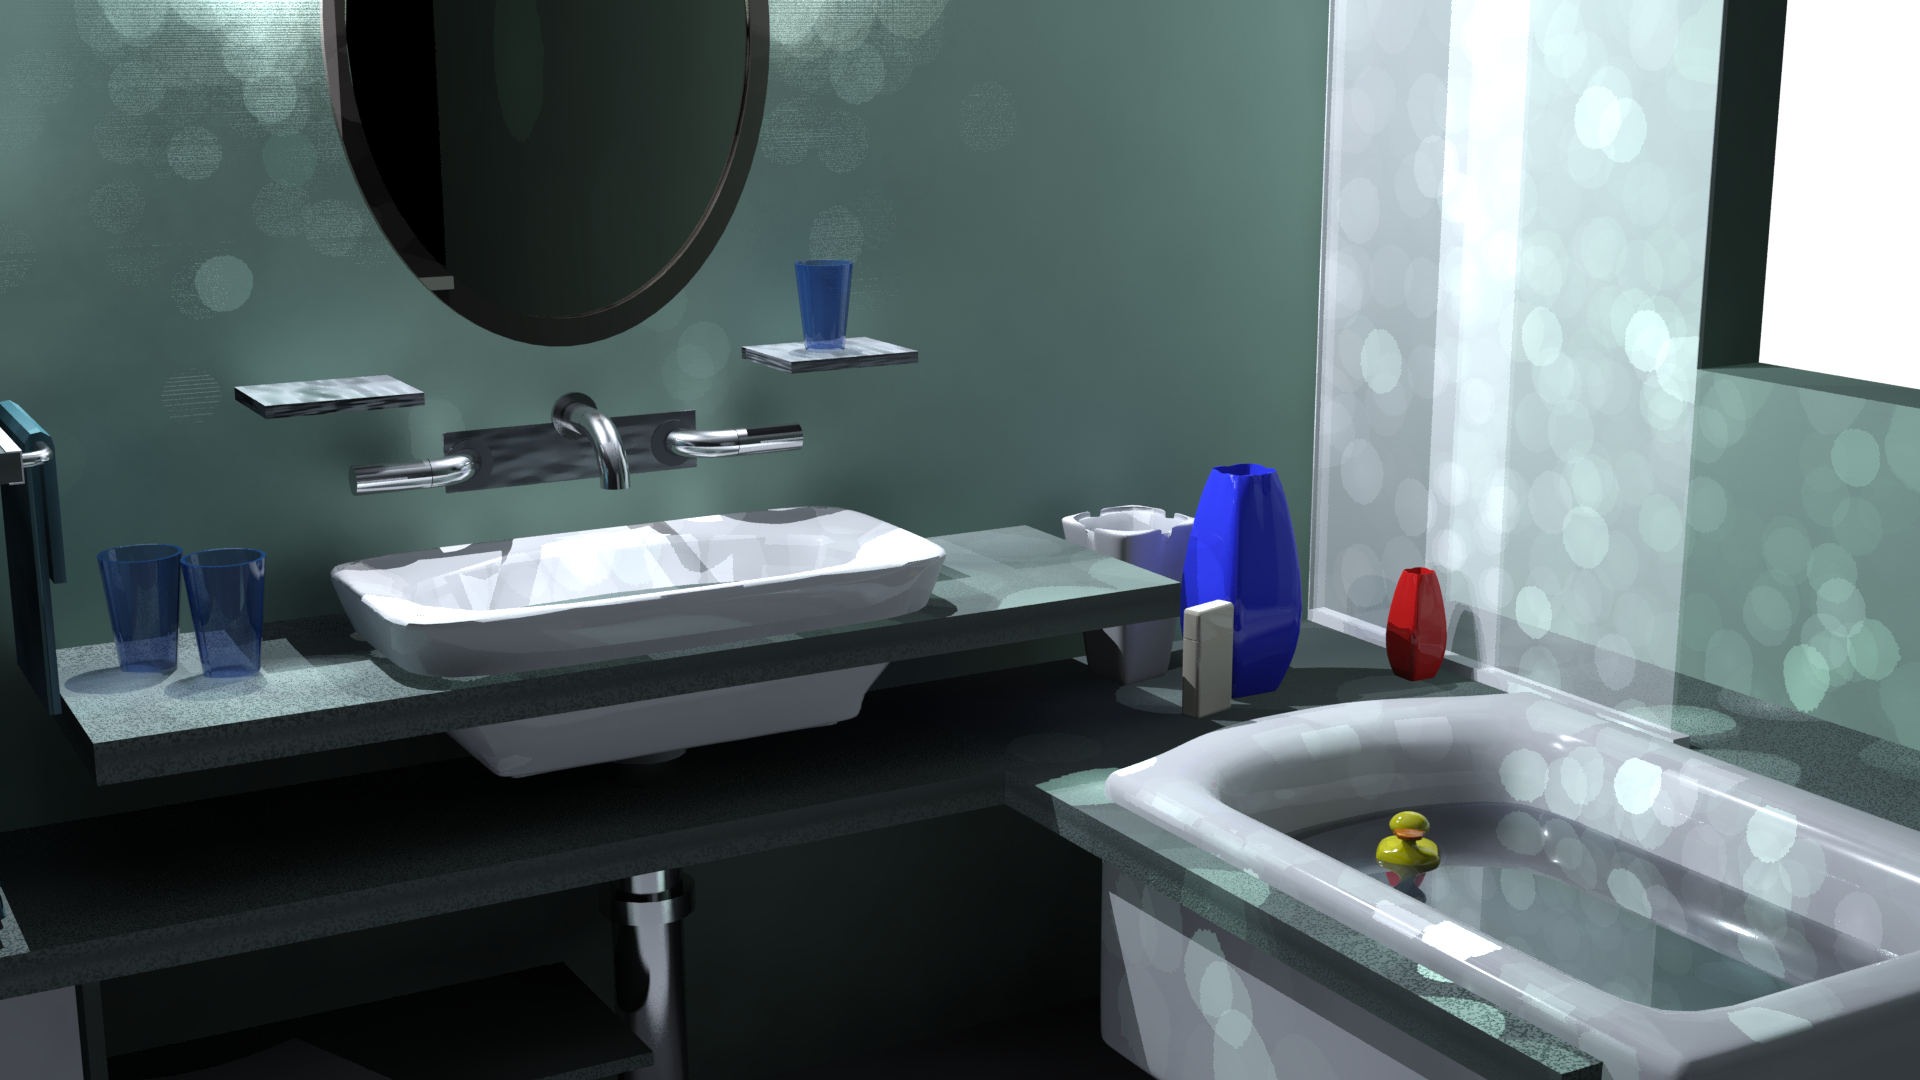
\includegraphics[width=10cm]{img/8000K.png}
	\caption{8000K}
	\label{fig:colortemp8000}
\end{figure}
\end{frame}
\begin{center}\line(1,0){250}\end{center}

\begin{frame}
\frametitle{15000 Kelvin}
\begin{figure}
	\centering
		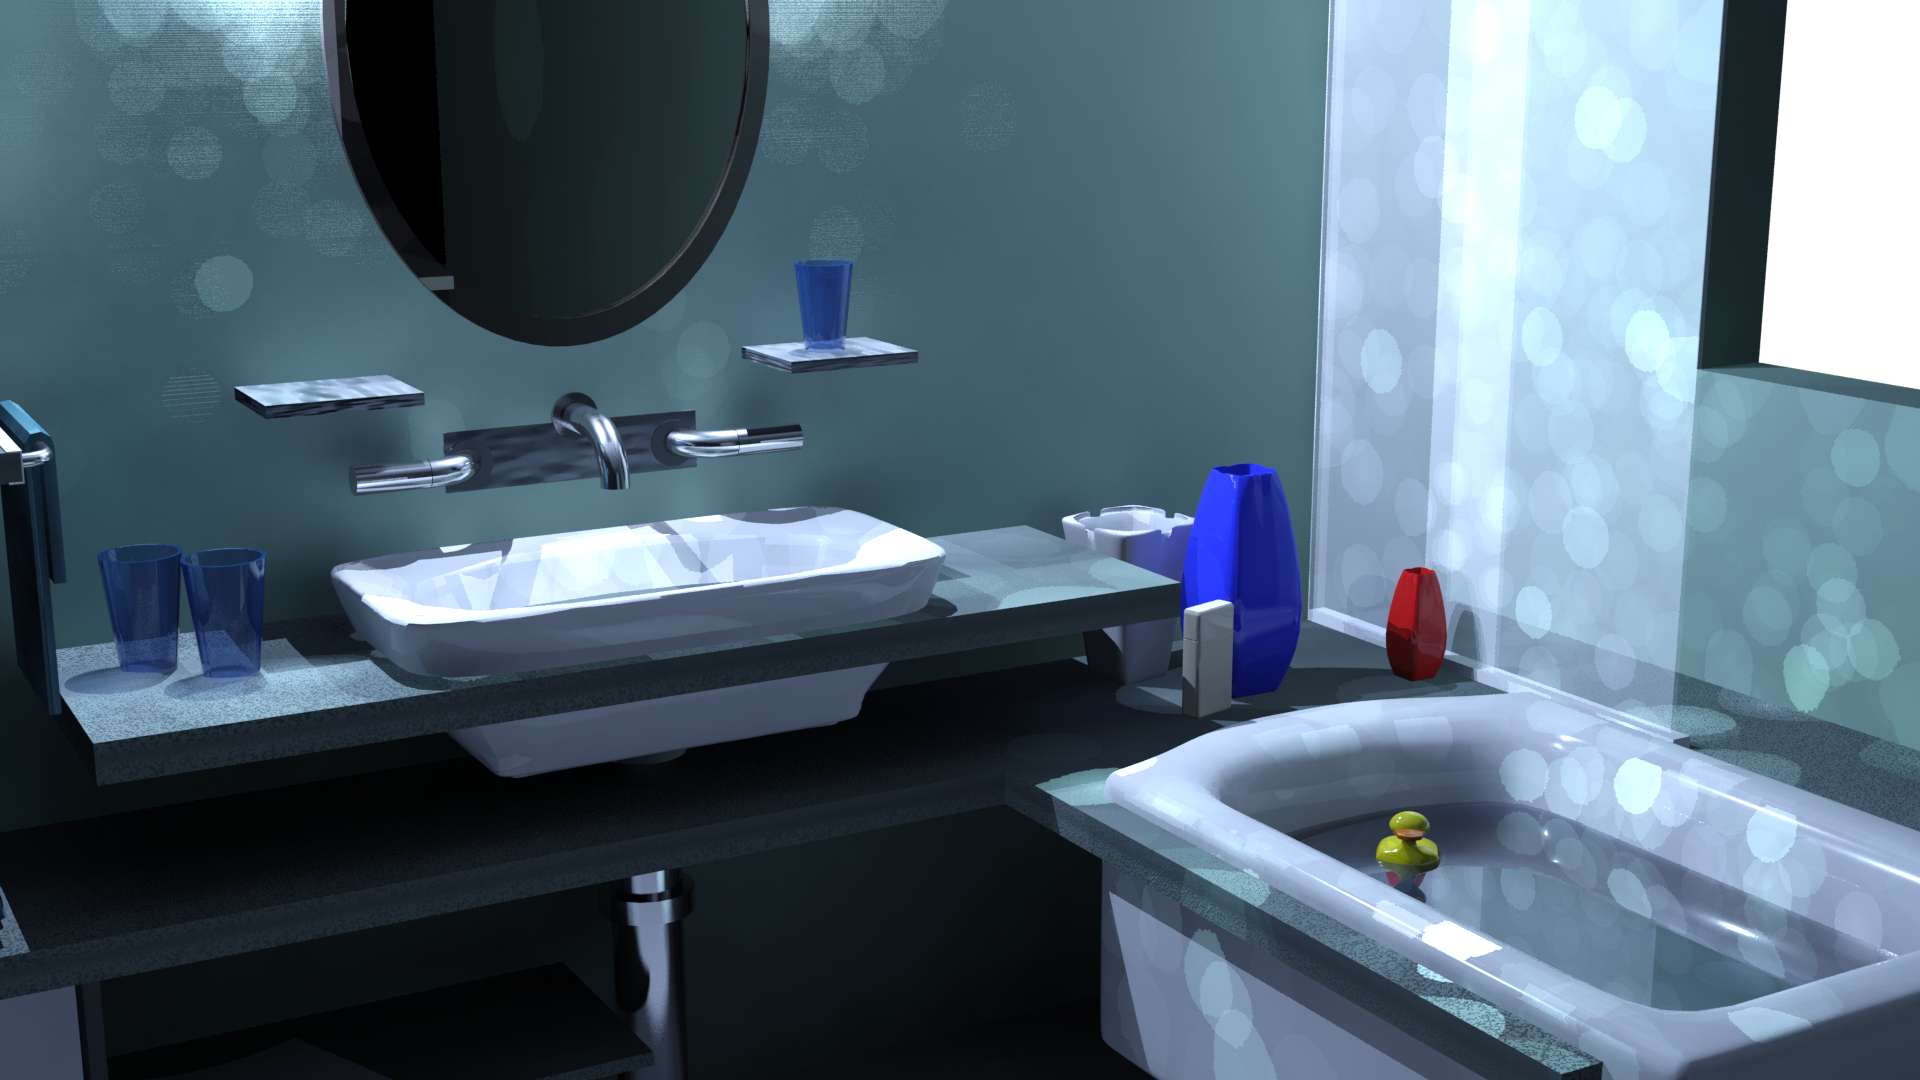
\includegraphics[width=10cm]{img/15000K.png}
	\caption{15000K}
	\label{fig:colortemp15000}
\end{figure}
\end{frame}
\begin{center}\line(1,0){250}\end{center}

\begin{frame}
\frametitle{Color Temperature}
\begin{itemize}
	\item Generally it is not a good idea to stray too far from the 4800-5000K range
	\item We can warm up, or cool down a scene by adjusting the color temperature up or down by 1000K
	\item Too much adjustment will force an artificial look on your image.
\end{itemize}
\end{frame}
\begin{center}\line(1,0){250}\end{center}



\section{State Sets}

\begin{frame}
\frametitle{State Sets}
\begin{itemize}
	\item Max provides us with the option of saving our models in various 'States' within the .max file
	\item It is extremely useful for keeping small adjustments within the model
	\item 'Manage State Sets' is available under the 'quad' menu.
	\item In the following images, state sets were used to retain material assignments for color options.
\end{itemize}
\end{frame}
\begin{center}\line(1,0){250}\end{center}


\begin{frame}
\frametitle{Base State}
\begin{figure}
	\centering
		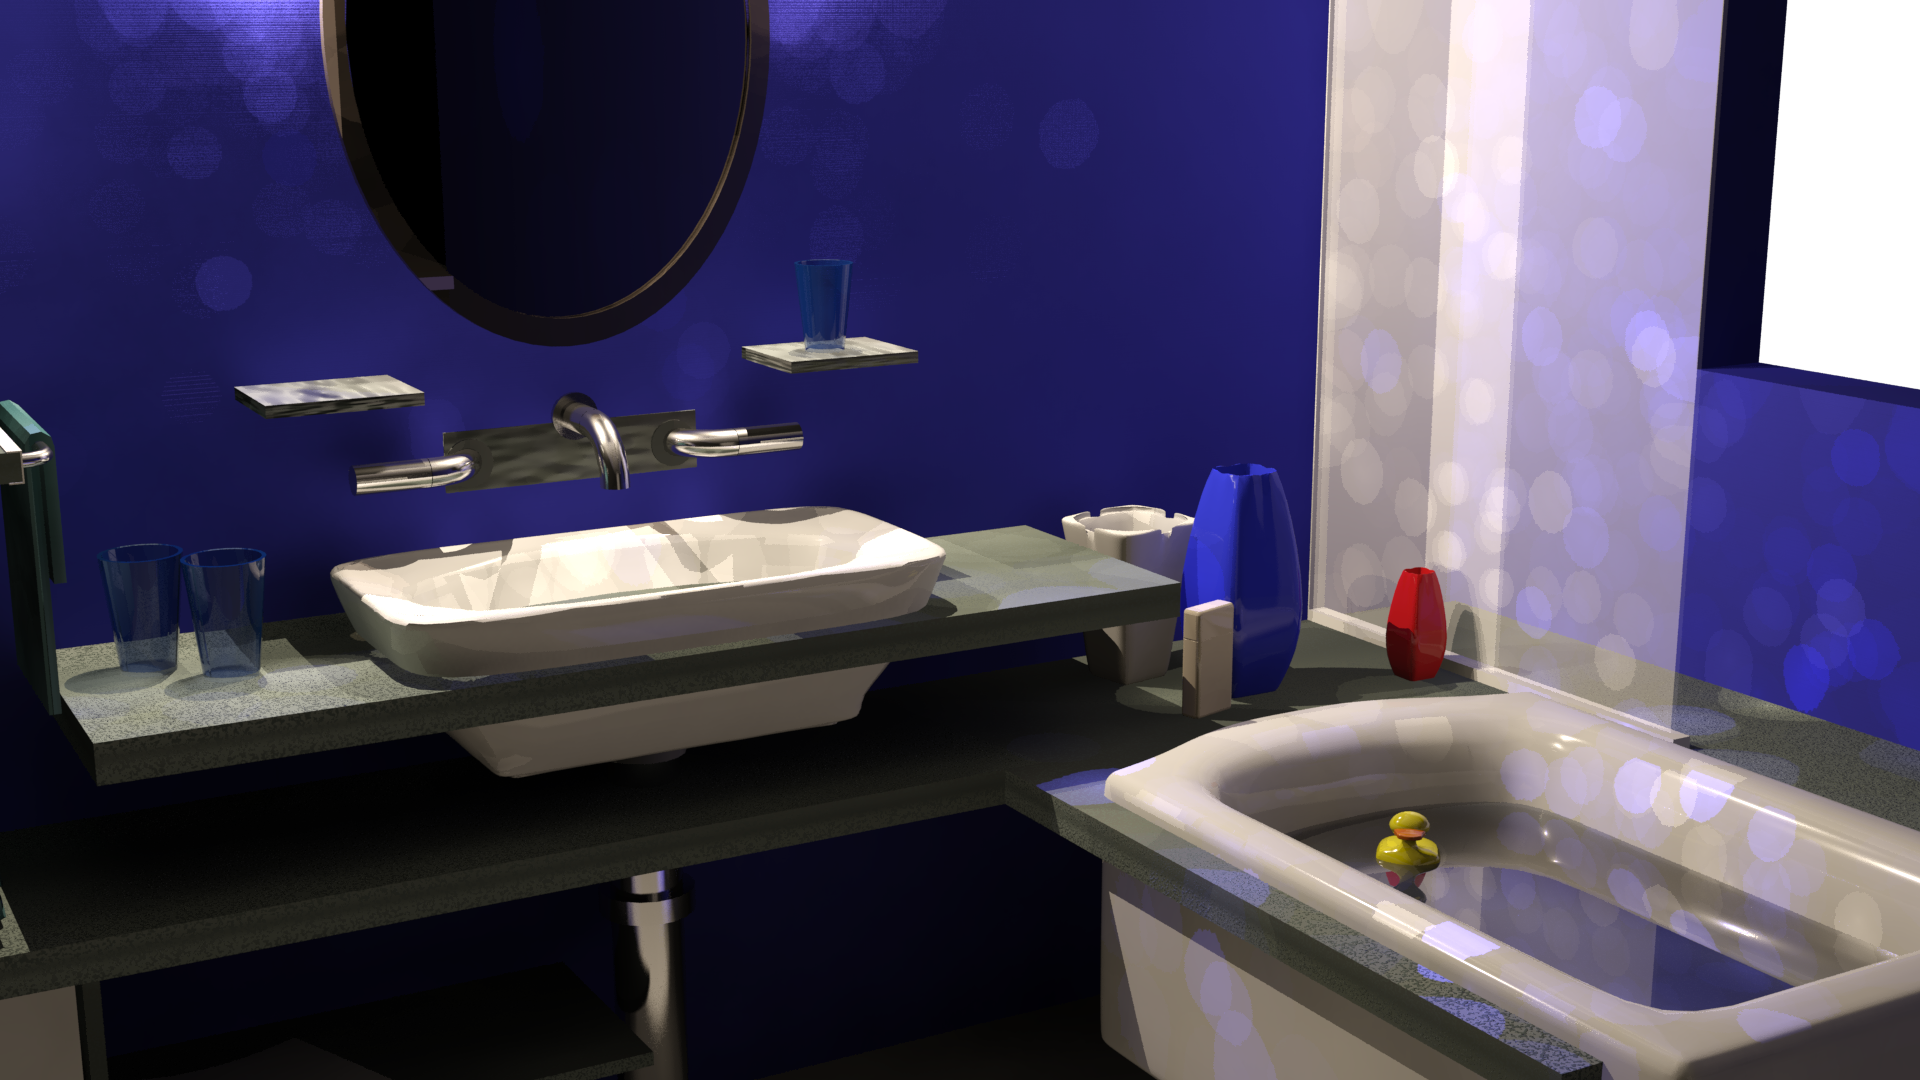
\includegraphics[width=10cm]{img/Base.png}
	\caption{Base State}
	\label{fig:BaseState}
\end{figure}
\end{frame}
\begin{center}\line(1,0){250}\end{center}

\begin{frame}
\frametitle{Yellow Paint}
\begin{figure}
	\centering
		\includegraphics[width=10cm]{img/yellow.png}
	\caption{Yellow State Set}
	\label{fig:yellow}
\end{figure}
\end{frame}
\begin{center}\line(1,0){250}\end{center}

\begin{frame}
\frametitle{Red Paint}
\begin{figure}
	\centering
		\includegraphics[width=10cm]{img/red.png}
	\caption{RedPaint State Set}
	\label{fig:RedPaint}
\end{figure}
\end{frame}
\begin{center}\line(1,0){250}\end{center}

\begin{frame}
\frametitle{Olive Green Paint}
\begin{figure}
	\centering
		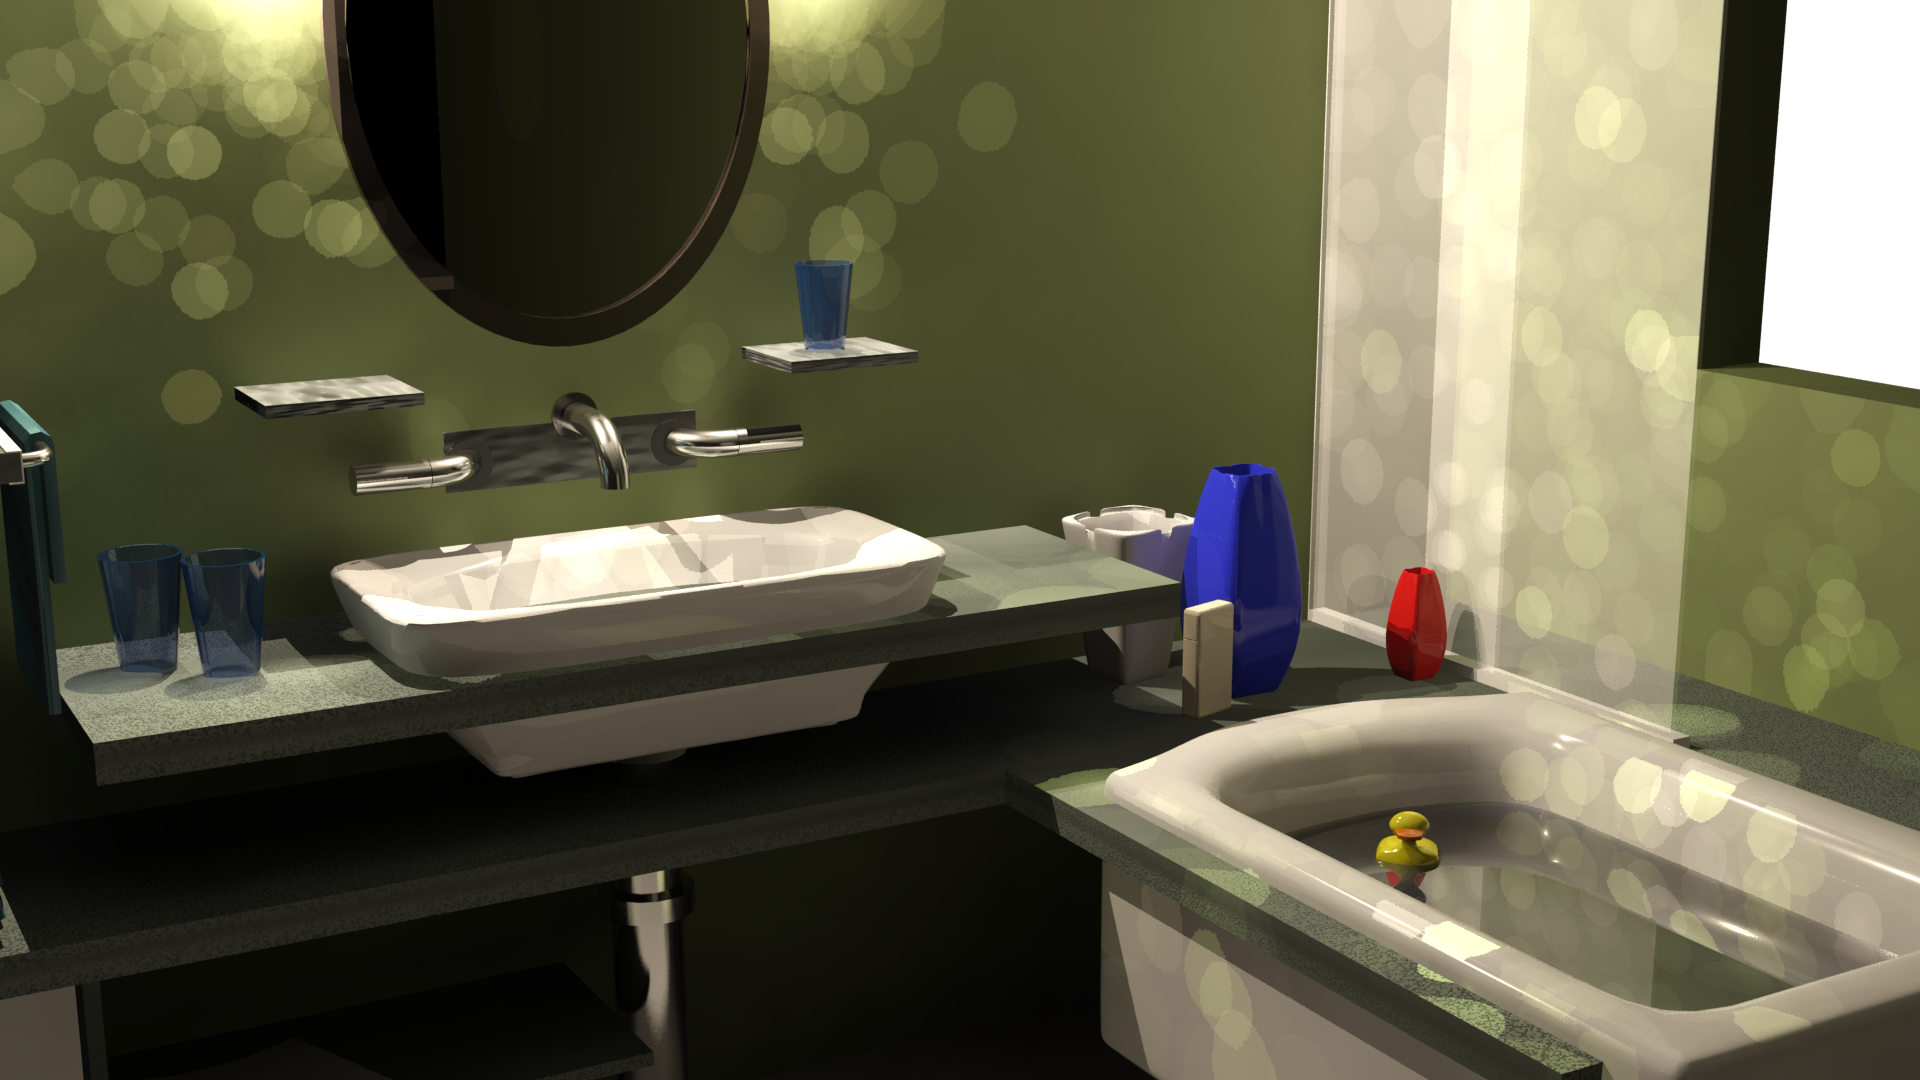
\includegraphics[width=10cm]{img/OliveGreen.png}
	\caption{OliveGreen State Set}
	\label{fig:OliveGreen}
\end{figure}
\end{frame}
\begin{center}\line(1,0){250}\end{center}


\begin{frame}
\frametitle{State Sets}
\begin{itemize}
	\item State sets are not limited to simple material changes
	\item Cameras, Materials, Geometery, Lights, and other scene attributes can be saved in a state set
	\item Used correctly state sets can greatly improve the speed of your workflow, and can be used for batch rendering.
\end{itemize}
\end{frame}
\begin{center}\line(1,0){250}\end{center}

\section{Rendering Engines}

\begin{frame}
\frametitle{Rendering Engines}
Max ships with a number of rendering engines
\begin{itemize}
	\item \textbf{Scanline} - poor quality, fast, good for checks, but not recommended
	\item \textbf{Mental Ray} - NVIDIA product, appropriate for production
	\item \textbf{IRay} - NVIDIA product, set to replace Mental Ray; Good for photoreal, quite slow on commodity hardware.
\end{itemize}
\end{frame}
\begin{center}\line(1,0){250}\end{center}



\begin{frame}
\frametitle{Scanline Image}
\begin{figure}
	\centering
		\includegraphics[width=10cm]{img/scanline.png}
	\caption{Scanline Renderer}
	\label{fig:Scanline}
\end{figure}
\end{frame}
\begin{center}\line(1,0){250}\end{center}



\begin{frame}
\frametitle{Mental Ray Image}
\begin{figure}
	\centering
		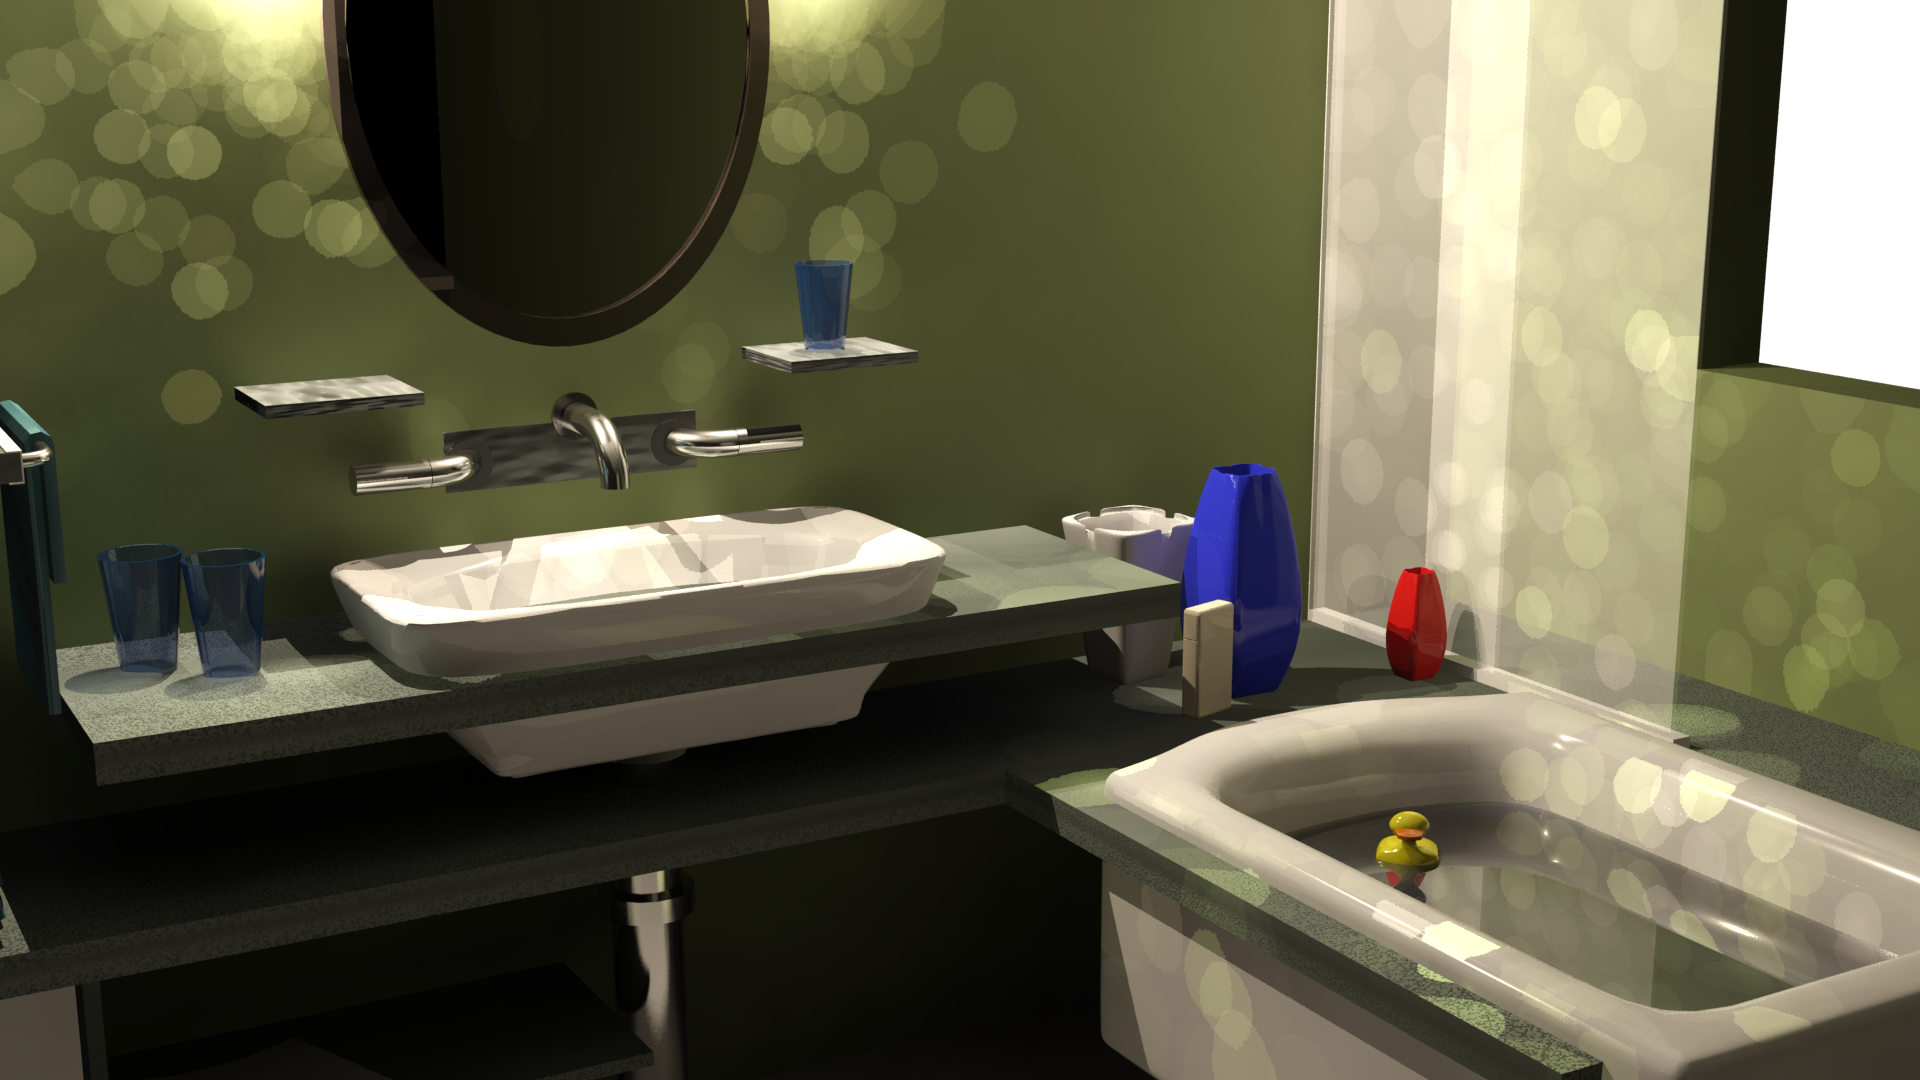
\includegraphics[width=10cm]{img/mentalray.png}
	\caption{Mental Ray Renderer}
	\label{fig:MentalRay}
\end{figure}
\end{frame}
\begin{center}\line(1,0){250}\end{center}



\begin{frame}
\frametitle{IRay image}
\begin{figure}
	\centering
		\includegraphics[width=10cm]{img/iray20min.png}
	\caption{IRay - note grey panel behind red vase}
	\label{fig:IRay}
\end{figure}
\end{frame}
\begin{center}\line(1,0){250}\end{center}


\begin{frame}
\frametitle{Rendering Engines and Materials}
\begin{itemize}
	\item Unfortunately, not all materials work with all rendering engines.
	\item Mental Ray supports features that IRAY does not.
	\item If IRAY cannot resolve a material correctly it will render it as gray.
\end{itemize}
\end{frame}
\begin{center}\line(1,0){250}\end{center}


\begin{frame}
\frametitle{Rendering Tweeks}
\begin{itemize}
	\item Ambient Occlusion - Mental Ray: adds soft shadows to small objects.  Adds richness to the image
	\item 
\end{itemize}
\end{frame}
\begin{center}\line(1,0){250}\end{center}





\section{Technology}


\begin{frame}
\frametitle{Rendering Engines}
3DS ships with two rendering engines
\begin{itemize}
	\item \textbf{Scanline:} Internal Autodesk, fast, generally poor quality, not recommended
	\item \textbf{Mental Ray:} by NVIDIA; better, good integration with 3DS.  Can use standard, autodesk or Mental Ray materials.  Good level of customization possible
\end{itemize}
Another Rendering Engine you will come across is \textbf{V-Ray}. This is the preferred option for most visualization houses due to its high levels of accuracy and third level support.  It is available to students at discounted rates; currently about \$200.00
\end{frame}
\begin{center}\line(1,0){250}\end{center}



\begin{frame}
\frametitle{Graphics Cards}
The graphics cards does most of the rendering work, and as such you need a good one to produce renders within a reasonable amount of time.  There are hundreds of graphics cards on the market, however you will find that most fall into one of two main options
\begin{itemize}
	\item NVIDIA
	\item Raytheon
\end{itemize}
Remember that NVIDIA is the creator of Mental Ray, so you will find that Mental Ray performs best with NVIDIA hardware.
\end{frame}
\begin{center}\line(1,0){250}\end{center}


\begin{frame}
\frametitle{Graphics Cards \hfill\hfill Things to watch for}
There are two main components of a graphics card that indicates its level of performance
\begin{itemize}
	\item Memory
	\item Number or graphics processors (GPUs)
\end{itemize}
Often people will select a card on memory alone; although important for CG work you also need more GPUs in order to crunch through the render calculations.  A good resource for comparing graphics cards is \href{http://www.videocardbenchmark.net/}{http://www.videocardbenchmark.net/}
\end{frame}
\begin{center}\line(1,0){250}\end{center}




\newpage

%
%This is some text 


\bibliographystyle{plainnat}
%\bibliographystyle{Classes/CUEDbiblio}
%\bibliographystyle{Classes/jmb}
%\bibliographystyle{Classes/jmb} % bibliography style
\nocite{*}
%\renewcommand{\bibname}{Bibliography} % changes default name References to Bibliography
\addcontentsline{toc}{chapter}{Bibliography}

\bibliography{refs/references} % References file

\newpage

\printindex
\newpage





\end{document}
